\documentclass[a4paper,12pt]{article}
\usepackage[paperwidth=210mm,paperheight=297mm,left=27mm,right=27mm,top=27mm,bottom=27mm]{geometry}

\usepackage{graphicx}
\usepackage{blindtext}
\usepackage{adjustbox}
\usepackage{natbib}
\usepackage{lipsum}

\usepackage{bibentry}

\bibliographystyle{jmr}

\title{EEGS - Introduction to Stata\thanks{Escola de Economia e Gestão, Universidade do Minho, Portugal}}
\date{May, 2021}
\author{Anabela Carneiro\\ U Porto
\and João Cerejeira \\ U Minho
\and Miguel Portela \\ U Minho 
\and Paulo Guimarães \\ Banco de Portugal \& U Porto}

\begin{document}

\maketitle

\section{Introduction}\label{sec:intro}

Figure \ref{fig:incdensity} sets the stage for our example, while Table \ref{tb:descriptives} shows descriptive statistics for the data used in the regression analysis. It shows a kerndel density for income. Table \ref{tb:regresults} presents our regressions. One could follow the book by \cite{acemoglu2016} to motivate the discussion. A thorough discussion of Econometrics is provided by \cite{greene2017} (see also \citep{verbeek2012}).\footnote{\cite{wooldridge2015introductory} makes a good introduction to Econometrics.}

\lipsum

\begin{table}[ht]
\begin{center}
\caption{Descriptive statistics}\label{tb:descriptives}
\resizebox{0.9\textwidth}{!}
	{{
\def\sym#1{\ifmmode^{#1}\else\(^{#1}\)\fi}
\begin{tabular}{l*{1}{cccc}}
\hline\hline
                    &        mean&          sd&         min&         max\\
\hline
Age (years)         &     39.2219&       3.038&       34.00&        46.0\\
Graduate            &      0.2481&       0.432&        0.00&         1.0\\
Union               &      0.2465&       0.431&        0.00&         1.0\\
Experience (years)  &     12.8413&       4.597&        0.12&        28.9\\
Tenure (years)      &      6.5710&       5.639&        0.00&        25.9\\
Working hours       &     37.6332&      10.064&        1.00&       100.0\\
Wage (log)          &      1.8962&       0.523&        0.30&         5.3\\
\hline
Observations        &        1870&            &            &            \\
\hline\hline
\end{tabular}
}
}
\end{center}
\end{table}

\lipsum

\lipsum

\begin{figure}[ht]
	\begin{center}
		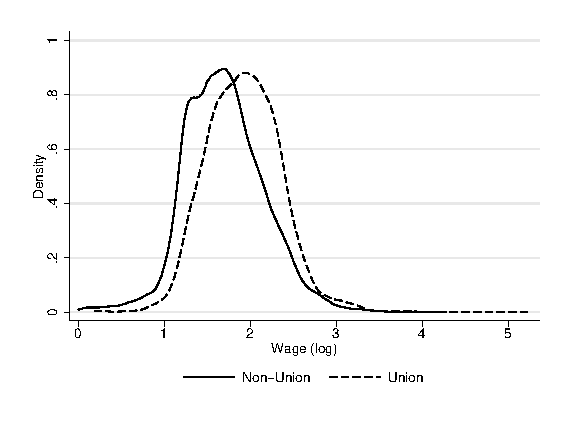
\includegraphics[scale = 0.9,trim = 0.0 0.0 0.0 0.0,clip]{figures/fig_wage_density_union.eps}
		\caption{Income density}\label{fig:incdensity}
	\end{center}
\end{figure}

\lipsum

\begin{table}[htbp]\centering
\def\sym#1{\ifmmode^{#1}\else\(^{#1}\)\fi}
\caption{Regression analysis -- Wages (logs)}
\begin{tabular}{l*{2}{c}}
\hline\hline
                    &         OLS         &          FE         \\
\hline
Experience (years)  &       0.051\sym{***}&       0.044\sym{***}\\
                    &     (0.001)         &     (0.002)         \\
[1em]
Union               &       0.189\sym{***}&       0.101\sym{***}\\
                    &     (0.007)         &     (0.007)         \\
\hline
Observations        &       19238         &       19238         \\
Firms               &                     &     4150.00         \\
R-sq-within         &                     &        0.14         \\
R-sq-between        &                     &        0.25         \\
Rho                 &                     &        0.69         \\
corr(u\_i,Xb)        &                     &        0.11         \\
\hline\hline
\multicolumn{3}{l}{\footnotesize Notes: robust standard errors in parenthesis (clustered at the sector level).}\\
\multicolumn{3}{l}{\footnotesize Significance levels: *, 10 %; **, 5 %; ***, 1 %.}\\
\multicolumn{3}{l}{\footnotesize All regressions include a constant and time dummies.}\\
\end{tabular}
\end{table}


\lipsum

\bibliography{references}

\end{document}
